\documentclass[numsec,webpdf,modern,large,numbered]{oup-authoring-template}

% Bioinformatics Application Note-style manuscript (content-structured).
% Generated from your Word draft; fill in TODO items before submission.

\usepackage{booktabs}
\usepackage{hyperref}
\usepackage{url}
\usepackage{microtype}
\usepackage{setspace}
\usepackage{xcolor}
\usepackage[switch]{lineno}
\setcitestyle{square,numbers,sort&compress}

\definecolor{revisionred}{RGB}{185,28,28}
\newcommand{\rev}[1]{\textcolor{revisionred}{#1}}

% Journal metadata (optional for submission; safe to leave as placeholders)
\journaltitle{Bioinformatics}
\pubyear{2026} % TODO
\copyrightyear{2026} % TODO
\appnotes{Applications Note}

\begin{document}

\firstpage{1}

\title[PyFgsea: Rust-powered fgseaMultilevel-aligned GSEA]{PyFgsea: A Rust-Powered, fgseaMultilevel-Aligned GSEA Framework with Rolling-Window Enrichment Along Single-Cell Trajectories}

\author{Kuanghao Wang\textsuperscript{1}}
\author{Hong Shi\textsuperscript{1,*}}

\address{\textsuperscript{1}Institute of Primate Translational Medicine, Kunming University of Science and Technology, Kunming 650500, China}

\corresp{*To whom correspondence should be addressed. Email: shih@kust.edu.cn}

\keywords{Gene set enrichment analysis; multilevel sampling; rare-event estimation; single-cell trajectories; Rust; PyO3}

\abstract{
\subheading{Summary:} \rev{GSEA is a standard approach for pathway interpretation, yet Python ecosystems lack a high-performance implementation aligned with the fgseaMultilevel rare-event estimator target, especially for trajectory-aware rolling-window analysis. PyFgsea achieves numerical alignment with the R fgseaMultilevel reference for normalized enrichment scores (NES; Pearson $r > 0.999$) and significantly reduces runtime compared to existing Python tools. Its stateful rolling-window engine further reduces repeated trajectory-analysis overhead, yielding approximately 1.9-fold end-to-end wall-time speedup in a conservative stress test and up to 7.47-fold component-level acceleration in a narrower 100-window benchmark.}
\subheading{Availability and implementation:} Source code is available at \href{https://github.com/shayuanxukuang/pyfgsea}{https://github.com/shayuanxukuang/pyfgsea} and via PyPI (\texttt{pip install pyfgsea}). \rev{An archival snapshot of the code and benchmark data is available on Zenodo (DOI: \href{https://doi.org/10.5281/zenodo.19446446}{10.5281/zenodo.19446446}).}
\subheading{Contact:} shih@kust.edu.cn
\subheading{Supplementary information:} Supplementary data are available at Bioinformatics online.
}

\maketitle

\doublespacing
\linenumbers

\section{Introduction}
Gene set enrichment analysis (GSEA) is widely used to interpret genome-wide expression profiles by quantifying whether a gene set is enriched toward the top or bottom of a ranked list \citep{Subramanian2005GSEA}.
In Python, commonly used implementations such as GSEApy \citep{Fang2023GSEApy} and BlitzGSEA \citep{Lachmann2022blitzGSEA} offer accessible workflows but may differ in runtime, memory, or the behaviour of extreme-tail $P$-values under multilevel sampling.

The \texttt{fgsea} R package provides an efficient multilevel adaptive sampling procedure (``fgseaMultilevel'') that targets accurate rare-event $P$-values without requiring extremely large numbers of permutations \citep{Korotkevich2021FGSEA}.
However, a statistically aligned, high-performance implementation has been missing from the Python ecosystem.
This gap becomes more pronounced in single-cell trajectory analysis, where enrichment is often desired along pseudotime using rolling windows, resulting in hundreds to thousands of GSEA evaluations.

We present PyFgsea, a high-performance framework built on a Rust backend with PyO3 bindings. \rev{To our knowledge, it fills a critical gap by providing: (i) a Python implementation aligned with the fgseaMultilevel rare-event estimator target; (ii) a multi-threaded architecture that substantially reduces runtime and memory footprint; and (iii) a specialized stateful rolling-window runner that minimizes redundant computations for efficient trajectory analysis.}

\section{Materials and Methods}
\subsection{Core multilevel workflow}
\rev{PyFgsea re-implements the fgseaMultilevel rare-event estimator target with the same ES definition, null-pathway construction, and multilevel tail factorization \citep{Korotkevich2021FGSEA}; in the current Rust release, the conditional levels are realized through empirical median thresholding and elite-clone rejuvenation. A complete methodological workflow diagram is provided in Supplementary Figure~S7.}
{\color{revisionred}
For a pathway $S$ of size $K$ in a ranked list of $N$ genes with ranked statistics $\{r_j\}$, PyFgsea uses the same weighted preranked enrichment score as in classical GSEA and fgseaMultilevel \citep{Subramanian2005GSEA,Korotkevich2021FGSEA}:
\[
ES=\max_{1\le i\le N}\left(P_{\mathrm{hit}}(i)-P_{\mathrm{miss}}(i)\right),\qquad
P_{\mathrm{hit}}(i)=\sum_{\substack{j\le i\\ j\in S}}\frac{|r_j|^{p}}{\sum_{g\in S}|r_g|^{p}},\qquad
P_{\mathrm{miss}}(i)=\sum_{\substack{j\le i\\ j\notin S}}\frac{1}{N-K}.
\]
The rare-event tail probability is then estimated through the same multilevel factorization \citep{Korotkevich2021FGSEA},
\[
P(ES\ge ES_{\mathrm{obs}})\approx P_0\prod_{l=1}^{L}P(ES\ge c_l\mid ES\ge c_{l-1}),
\]
using an initial baseline sample followed by progressively more extreme conditional levels. The current release therefore combines a baseline sample, empirical median-conditioned levels, elite-clone rejuvenation, and budget/precision/floor-based stopping.}
The Python API adheres to standard GSEA conventions: users provide ranked genes, a GMT gene set collection, and parameters controlling multilevel estimation (e.g., \texttt{eps}, \texttt{sample\_size}, \texttt{seed}).
\rev{PyFgsea differs primarily at the implementation layer (Rust/PyO3 backend, Rayon scheduling, deterministic pathway-local PRNG streams) and in the functional extension of a stateful rolling-window runner for trajectory analysis; Supplementary Table~S5 and Section~S8 provide a concise same-versus-different summary and fuller algorithmic details.}

\subsection{Rust backend and parallelism}
The computational core is implemented in Rust and exposed to Python via PyO3.
\rev{Pathway-level evaluations are parallelized across threads using a dynamic work-stealing strategy. To guarantee deterministic reproducibility across thread counts under matched inputs and a fixed master seed without synchronization blocking, PyFgsea derives independent, deterministic pseudo-random number generator (PRNG) streams for each pathway by hashing a user-provided global master seed with the unique pathway identifier (see Supplementary Section~S9).}
Memory allocations are minimized by reusing buffers across pathways and windows.
This design targets both speed and reduced peak RAM for large gene-set collections.

\subsection{Rolling-window GSEA for single-cell trajectories}
For trajectory analysis, PyFgsea supports rolling-window enrichment along pseudotime.
Cells are ordered by pseudotime (e.g., diffusion pseudotime, DPT \citep{Haghverdi2016DPT}) computed using Scanpy \citep{Wolf2018Scanpy}.
A window of fixed size slides along the ordered cells with a user-defined step size.
\rev{Trajectory termini are handled without padding, and Supplementary Figure~S14 additionally audits an explicit terminal-truncation extension. The choice of window and step size governs temporal resolution and statistical stability. As a practical starting range that should be tuned to trajectory length and noise level, we suggest an initial window size spanning 5--10\% of the total cells and a step size of 1--2\% of total cells. Smaller windows may be overly sensitive to single-cell noise, while excessively large windows risk oversmoothing biologically transient dynamics (a comprehensive parameter sensitivity analysis is provided in Supplementary Figure~S8 and Sections~S10 and S13). The erythroid illustration in Figure~2 intentionally uses a somewhat larger 500-cell baseline window (approximately 14\% of that analyzed trajectory) because this lineage segment is relatively short and noisy, and the figure prioritizes a smoother descriptive profile over maximal temporal resolution.}
For each sliding window along the pseudotime-ordered cells, we rank genes by a logFC-like score computed on log1p-normalized expression: $S_g = \mu_{g,in} - \mu_{g,out}$, where $\mu_{g,in}$ and $\mu_{g,out}$ denote mean expression of gene $g$ inside the current window and in all remaining cells, respectively.
The ranked list is then used as input to preranked GSEA over a chosen gene-set collection (e.g., MSigDB Hallmark \citep{Liberzon2015Hallmark,Liberzon2011MSigDB}).
\rev{Within each window, Benjamini--Hochberg adjustment is applied across pathways, so window-level significance corresponds to within-window FDR control. The rolling-window workflow is implemented in \texttt{pyfgsea.trajectory.run\_trajectory\_gsea}, and the repository includes a demonstrative script at \texttt{examples/trajectory\_demo.py} (release tag: \texttt{v0.1.4}).}

\subsection{Datasets and benchmarking}
We evaluated performance and faithfulness on both bulk-like and single-cell settings.
For single-cell demonstrations we used Human Cell Atlas (HCA) datasets \citep{Regev2017HCA} accessed through \texttt{HCAData} \citep{Marini2020HCAData}.
Benchmarking compared PyFgsea with GSEApy \citep{Fang2023GSEApy}, BlitzGSEA \citep{Lachmann2022blitzGSEA}, and the reference R \texttt{fgsea} implementation \citep{Korotkevich2021FGSEA} under matched inputs and parameters (see Supplementary Material for detailed parameter alignment).

Benchmarks were conducted on a server equipped with dual Intel Xeon Platinum 8352Y CPUs (64 cores/128 threads, @2.20GHz) and 1.5 TiB RAM, running Ubuntu 22.04.1 LTS.
Software versions were Python 3.10.19, R 4.4.3 (fgsea 1.32.2), GSEApy 1.1.11, and BlitzGSEA 1.3.54.
To ensure fairness, multithreading was controlled: PyFgsea and Python baselines used 4 threads (via \texttt{RAYON\_NUM\_THREADS=4} or \texttt{OMP\_NUM\_THREADS=4}), while R/fgsea was configured with \texttt{nproc=4} (using \texttt{BiocParallel}).
Each condition was measured in 3 independent repeats using independent processes to minimize cache interference.
Runtime and peak memory (PeakRSS) were recorded via \texttt{/usr/bin/time -v} or internal timers, reported as mean of 3 repeats in Supplementary Table S4.
Detailed performance breakdowns, including thread scaling and rolling-window component analysis, are provided in the Supplementary Material.

\section{Results}
\subsection{Performance and memory footprint}
Across representative dataset sizes (spanning small, medium, and large scales), PyFgsea consistently reduced runtime while using substantially less memory than alternative Python implementations \rev{(Supplementary Table~S4)}.
{\color{revisionred}In the large benchmark (20k genes, 5k gene sets), PyFgsea completed in 1.35~s with 68.0~MB PeakRSS, compared with 18.00~s and 611.4~MB for BlitzGSEA and 189.42~s and 5891.1~MB for GSEApy.}
These gains are primarily attributable to the Rust backend, pathway-level parallelism, and careful reuse of intermediate buffers.

\subsection{Statistical faithfulness to fgseaMultilevel}
To assess equivalence to the reference implementation, we compared enrichment scores (ES) and normalized enrichment scores (NES) against R \texttt{fgseaMultilevel} \citep{Korotkevich2021FGSEA}.
\rev{We observed near-identical ES/NES across a wide range of pathways (Figure~\ref{fig:accuracy}), achieving rigorous quantitative concordance with the R reference (Pearson $r=1.000$; Spearman $\rho=1.000$; RMSE $=0.0135$; median absolute difference $|\Delta|=0.0070$ for NES; Figure~1C). ES values were numerically identical within machine precision. Transformed nominal $P$-values remained overall concordant with the reference implementation (overall Pearson $r=0.997$; Spearman $\rho=0.988$; RMSE $=0.1696$; median $|\Delta|=0.0467$ on $-\log_{10}P$), although sparse local trajectory windows could show visibly larger dispersion than ES or NES (worst-window Pearson $r=0.941$ on $-\log_{10}P$; Supplementary Table~S7). In such sparse local windows, ES and NES should therefore be regarded as the primary cross-implementation comparanda, whereas transformed nominal-$P$ agreement is more sensitive to tail-estimation noise and pathway-count filtering.}
For multilevel $P$-values, PyFgsea employs a stricter default floor (\texttt{eps=1e-50}) compared to R's default (\texttt{eps=1e-10}), allowing for higher resolution in extreme tails.
\rev{When \texttt{eps} is matched, deep-tail $P$-value differences are generally modest, but they become more apparent when few pathways pass size filters or when strongly enriched local windows occupy sensitive rare-event tails (Supplementary Figures~S3 and S4).}
\rev{PyFgsea thus preserves ES within machine precision and NES near-identically relative to the reference procedure while offering extended precision for rare events.}

\begin{figure*}[!t]
\centering
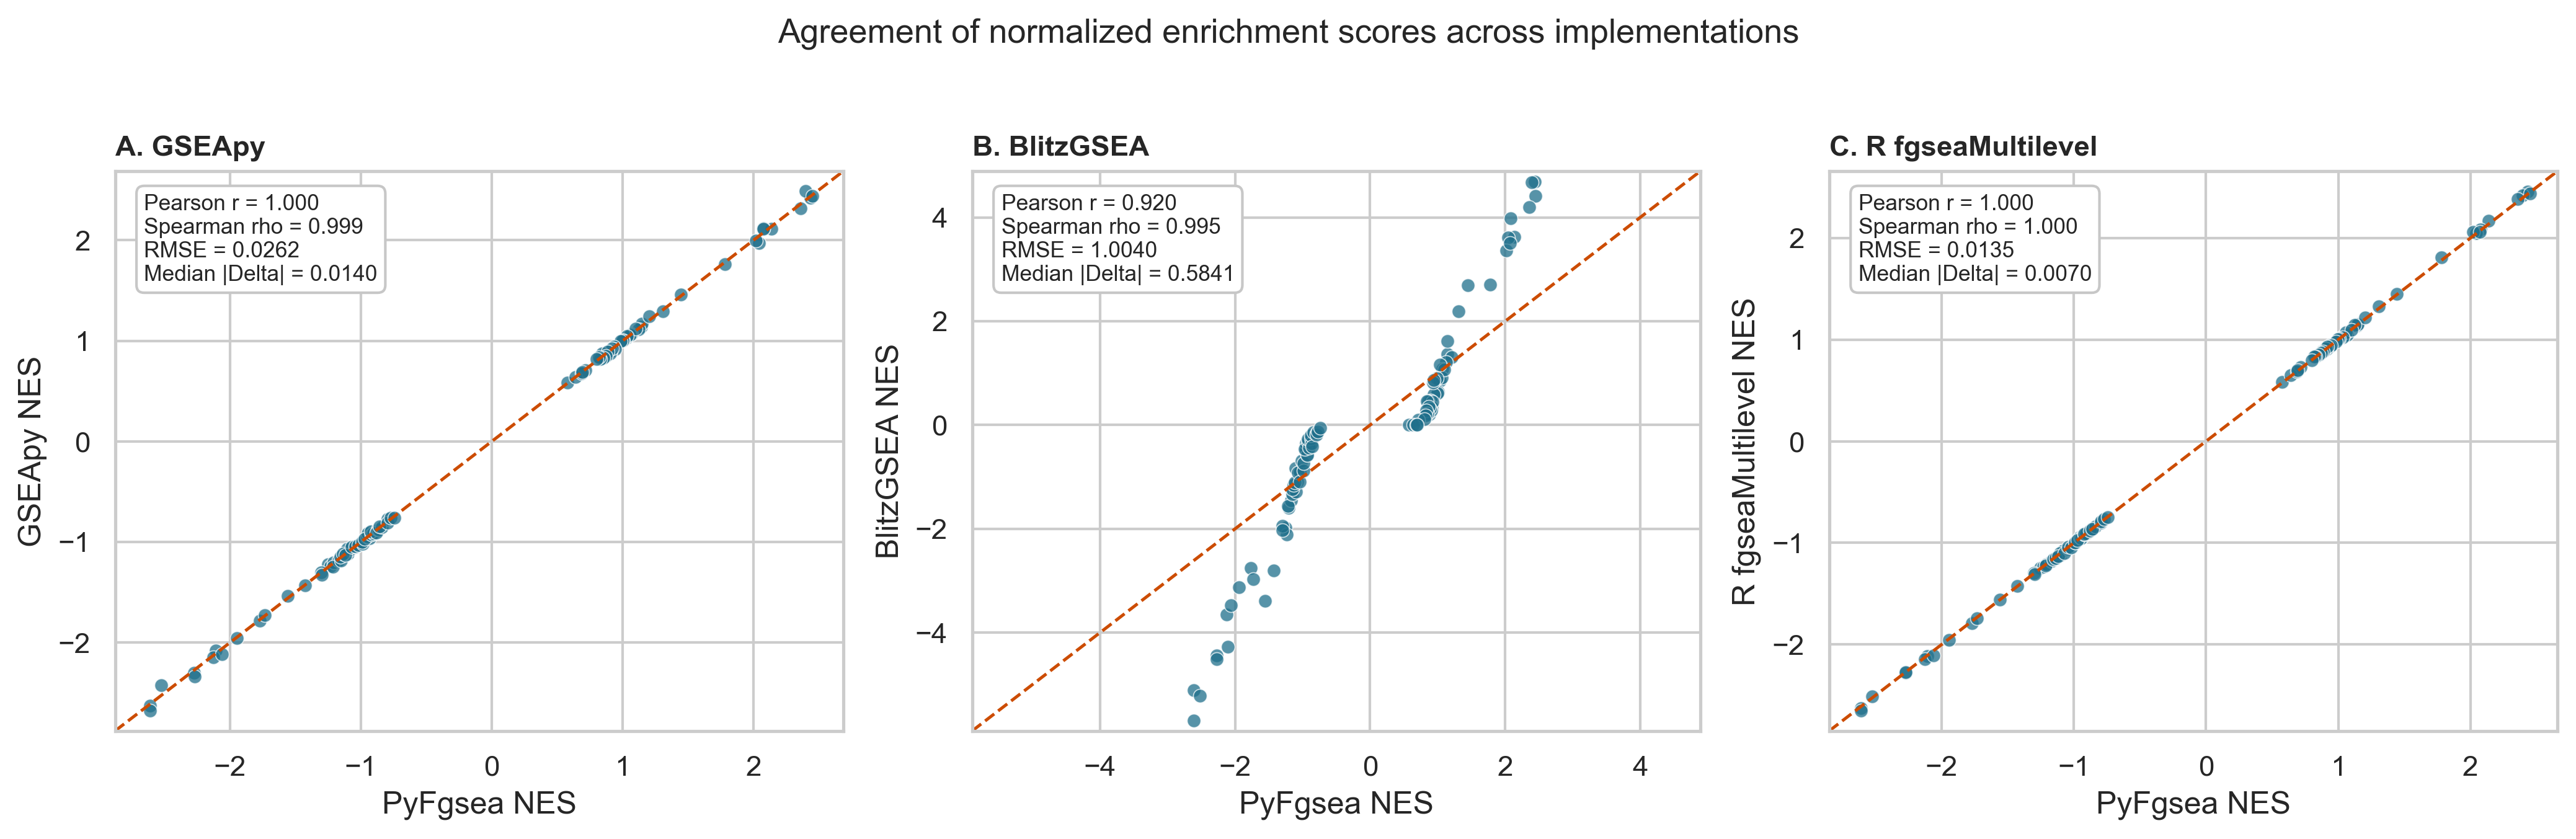
\includegraphics[width=0.80\textwidth]{figure1_agreement.png}
\caption{\rev{Agreement of normalized enrichment scores (NES) across implementations on matched synthetic benchmark inputs. Panels compare PyFgsea with (A) GSEApy, (B) BlitzGSEA, and (C) R fgseaMultilevel. Dashed lines indicate identity; insets report concordance statistics. PyFgsea is near-identical to the R reference.}}
\label{fig:accuracy}
\end{figure*}

\subsection{Trajectory case study: rolling-window enrichment}
PyFgsea enables rolling-window enrichment along pseudotime for large single-cell datasets.
\rev{In a real GSE155254-derived HSC-like-to-erythroid trajectory, windowed enrichment identified temporally localized pathway activation patterns while maintaining feasible runtimes over hundreds to thousands of windows (Figure~\ref{fig:trajectory}).}
\rev{Across rolling-window benchmarks, the stateful runner yielded approximately 1.9-fold speedup in a conservative end-to-end stress test and up to 7.47-fold acceleration in a narrower 100-window component benchmark.}
\rev{Figure~\ref{fig:trajectory} uses the default full-window workflow without the optional terminal-truncation extension, which is evaluated separately in Supplementary Figure~S14.}


\begin{figure*}[!t]
\centering
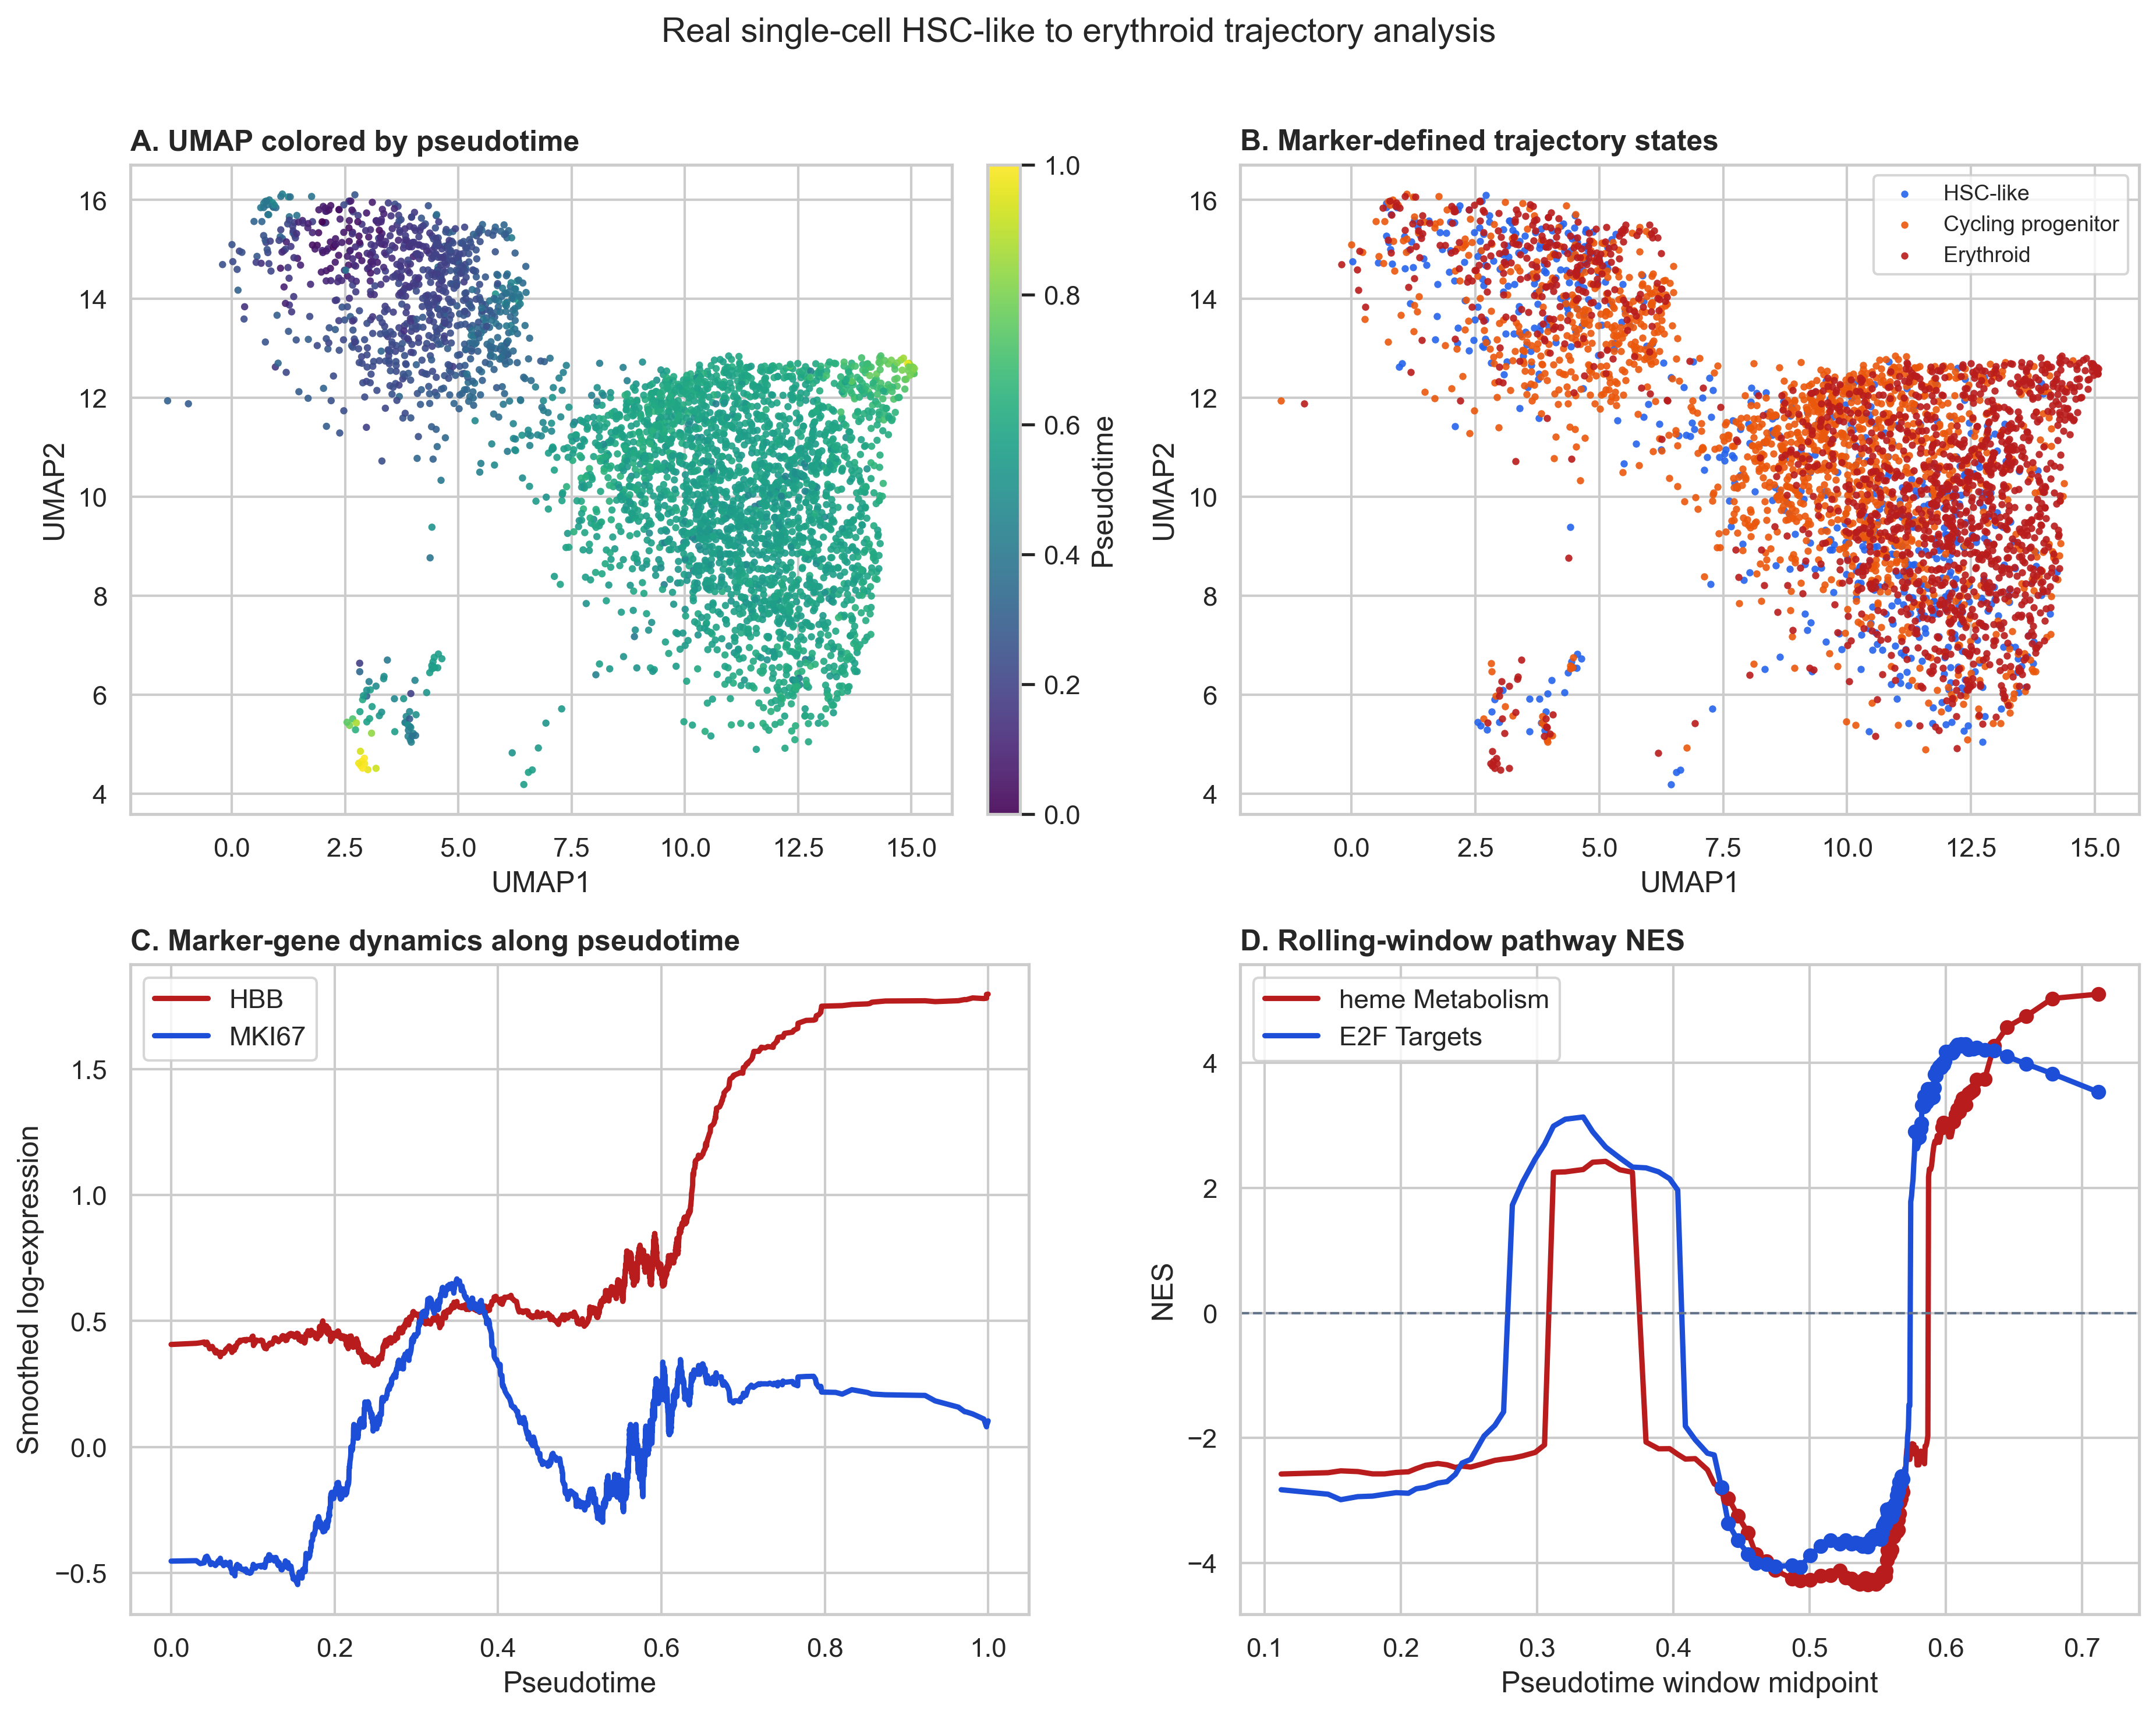
\includegraphics[width=0.95\textwidth]{figure2_real_trajectory.png}
\vspace{-15pt}
\caption{\rev{Rolling-window GSEA along a GSE155254-derived HSC-like-to-erythroid trajectory. (A) UMAP colored by diffusion pseudotime. (B) Marker-defined states. (C) Smoothed HBB and MKI67 expression. (D) Window-wise NES for representative pathways; filled points mark within-window FDR $< 0.05$ after Benjamini--Hochberg correction across pathways. The default full-window workflow is shown; terminal-truncation is audited in Supplementary Figure~S14.}}
\label{fig:trajectory}
\vspace{-10pt}
\end{figure*}

\section{Discussion}
PyFgsea brings an fgseaMultilevel-aligned multilevel estimator to the Python ecosystem and extends it to rolling-window trajectory analysis.
\rev{When interpreting trajectory dynamics, users should be mindful of the inherent limitations of the rolling-window ranking statistic. By summarizing local expression changes as a simple difference of means, it inherently assumes monotonic expression shifts within the evaluated window. Consequently, genes exhibiting complex, non-monotonic dynamics outside the local window may have their relative changes underestimated, potentially causing false-negative enrichments. Conversely, sparse genes with high technical variance may dominate local rankings, risking false positives. We recommend interpreting dynamic pathways cautiously and cross-referencing with smoothed single-gene visualizations.}

Future work includes broader input conventions, additional trajectory ranking statistics, and more diverse cross-platform validation.

\section*{Availability and implementation}
PyFgsea is released under the MIT License. Source code, documentation, and tutorials are available at \href{https://github.com/shayuanxukuang/pyfgsea}{https://github.com/shayuanxukuang/pyfgsea}. The Python package can be installed directly from PyPI (\texttt{pip install pyfgsea}) and supports Linux, Windows, and macOS. \rev{A permanent archival snapshot is also available at Zenodo: \href{https://doi.org/10.5281/zenodo.19446446}{10.5281/zenodo.19446446}.}


\section*{Data availability}
\rev{All scripts and minimal example data required to reproduce the reported software benchmarks and rolling-window workflow are provided in the public PyFgsea repository under \texttt{repro/}, \texttt{examples/}, and the package source tree (\textit{see Availability and implementation}).}
Public reference resources used in the showcase analyses include Human Cell Atlas datasets (accessed via \texttt{HCAData}) and MSigDB hallmark gene sets; access and licensing follow the respective \rev{providers' terms}.


\section*{Author contributions}
K.W.\ implemented the software and performed experiments. H.S.\ supervised the project and contributed to manuscript editing. All authors approved the final manuscript.

\section*{Conflict of interest}
None declared.

\section*{Funding}
None declared.

\bibliographystyle{unsrtnat}
\bibliography{references}

\end{document}
